\chapter{Metodologie}
\label{cap:nomePrimoCapitoloTesi}
\lhead{\textbf{\rightmark}}

\indent{
Il significato della diagnosi precoce del melanoma ha motivato lo sviluppo di sistemi di rilevamento/classificazione (CAD) assistiti da computer/server.
\newline 
La comunità scientifica continua a lavorare verso il miglioramento delle prestazioni diagnostiche e l'integrazione clinica della tecnologia CAD mobile.
Per questo motivo, è necessario che i sistemi CAD siano affidabili per la rilevazione/classificazione automatizzata delle lesioni del melanoma e saranno molto utili per fornire una preziosa "seconda opinione" al controllo del melanoma durante la visita dermatologica.

Dopo aver effettuato una revisione dettagliata delle tecniche e dei sistemi CAD correlati al rilevamento da smarphone o dispositivo mobile del melanoma (questa revisione includeva metodi e tecniche) si è scelto di utilizzare un approccio gerarchico (già utilizzato da altri sistemi), applicando prima passaggi di pre-elaborazione (o preprocessing) delle immagini per migliorare le strutture sospette nell'immagine e quindi impiegando l'estrazione delle caratteristiche e infine la classificazione come valutazione del nevo per indicare la presenza o meno di un melanoma. La visione delle informazioni e del livello di classificazione sarà in realtà aumentata, attraverso continous analysis e tracking del nevo.
\newline
In particolare questo lavoro si concentra sul testare ed esaminare un nuovo sistema per migliorare i seguenti aspetti:
\begin{itemize}
	\item pre-elaborazoine e miglioramento dell'immagine;
	\item pulizia dell'immagine da eventuali peli e/o imperfezioni;
	\item segmentazione accurata del nevo;
	\item feature extaction vettoriale e valutazione delle metodologie applicate per l'estrazione;
	\item visione dei risultati in realtà aumentata.
\end{itemize}
L'obiettivo finale è costruire un sistema mobile più robusto e implementarlo su un ambiente mobile/server per espandere le possibilità del sistema nell'acquisizione ed elaborazione precisa e dettagliata delle immagini.
\newline
Questo sistema faciliterà l'analisi del melanoma e fornirà la visione delle informazioni in realtà aumentata, cosicché il dermatologo o persona addetta all'analisi dei nevi potrà usufruire di un sistema robusto ed efficace ma che non va a sostituire il ruolo del medico dermatologo nell'analisi ma funge solo da supporto ad esso.
\newline
\section{Approccio proposto}
Allo stato dell'arte per la definizione dell'architettura di sviluppo in questo lavoro, ci si basa sulle attività di ricerca per l'analisi, la valutazione e il rilevamento del melanoma utilizzando la tecnologia mobile e tecniche di classificazione basate su \textit{feature extraction and classification}.\cite{mackinnon2016melanoma, taufiq2017m, chao2017smartphone, kleinjan2017introducing}
\newline
La Figura sottostante mostra l'approccio proposto.
\begin{figure}[h]
	\begin{center}
		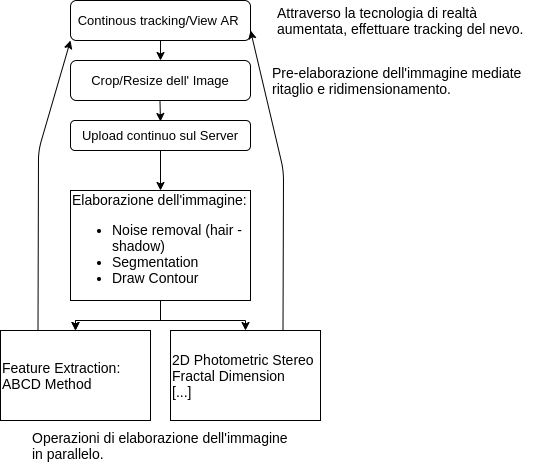
\includegraphics[scale=0.75]{figure/capitolo4/architettura.png}
	\end{center}
	\caption{Architettura di sistema ad alto livello per l'analisi dei nevi e visione in AR}	
\end{figure}
\newline
L'obiettivo di questo lavoro è testare una serie di algoritmi per il rilevamento del melanoma su un ambiente mobile/server, inviando continuamente dati ed informazioni al server; gli algoritmi di rilevamento del melanoma si basano sull'elaborazione di immagini digitali, sull'estrazione delle caratteristiche e sulle tecniche di classificazione; in questo modo sarà possibile effettuare analisi complete e visualizzare gli elementi elaborati in realtà aumentata con una latenza il più bassa possibile.
\newline
\textit{L'obiettivo ultimo è poter dare al dermatologo la possibilità di effettuare analisi di un nevo con diverse prospettive di visione garantite dalla \textbf{realtà aumentata}.}
\newline
L'approccio proposto in AR consiste nelle seguenti fasi:
\begin{enumerate}
	\item Attività di continous tracking in cui il nevo da analizzare viene in tempo reale ricercato;
	\item Taglio e ridimensionamento dell'immagine;
	\item Upload sul server;
	\item Elaborazione dell'immagine (Preprocessing);
	\item Feature Extraction:
	\subitem ABCD Method;
	\subitem 2D Photometric Stereo;
	\subitem Fractal Dimension;
	\item Valutazione del classificatore;
	\item Invio dei dati al dispositivo;
	\item Visualizzazione dei dati in Realtà Aumentata;
	\item Torna al passo 1.
\end{enumerate}
\newpage
\section{Image Preprocessing}
L'elaborazione delle immagini include molti dettagli:
\begin{enumerate}
    \item Acquisizione delle immagini utilizzando uno smartphone mobile;
    \item Pre-elaborazione delle immagini;
    \item Invio al server;
    \item Pre-processing dell'immagine (Image Pre-processing);
    \item Segmentazione;
    \item Estrazione delle caratteristiche;
\end{enumerate}
\subsection{Image Capture / Continous Tracking}
L'interfaccia di analisi deve essere semplice e pensata seguendo un approccio di utilizzo semplificato basato sui sette principi di Norman.\cite{houser1998learning}
\newline
Il \textit{continous tracking}, alla base dell'applicazione AR, permette al medico di effettuare analisi continuative sul medesimo nevo.
Il nevo dev'essere collocato al centro dell'immagine come in figura 5.2 dal dermatologo che può migliorarne la visione utilizzando il flash oppure aumentarne la dimensione attraverso lo zoom digitale.
\newpage
\subsection{Crop/Resize Image}
Prima di inviare il frame al server, questo deve essere ritagliato (crop), in modo da ridurre l'immagine e rendere il caricamento e l'analisi più veloce.
\begin{figure}[h]
	\begin{center}
		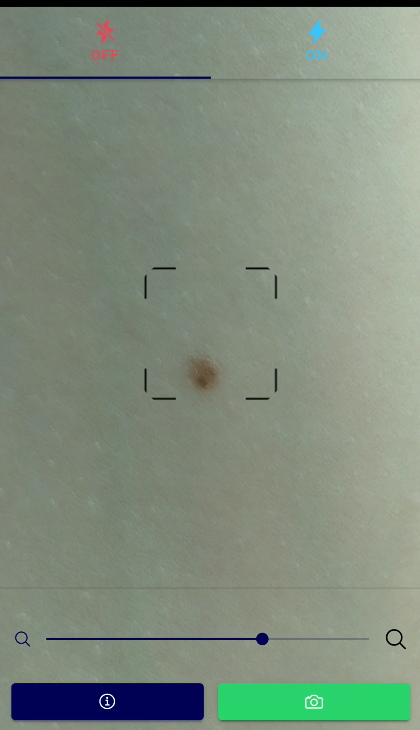
\includegraphics[scale=0.7]{figure/capitolo4/interface.png}
	\end{center}
	\caption{Esempio di interfaccia iniziale semplificata.}	
\end{figure}
\newpage
\subsection{Rimozione Peli}
Come alcune ricerche suggeriscono \cite{chatterjee2019integration, gutierrez2017skin}, il primo step del preprocessing dell'immagine per l'elaborazione di un melanoma è la rimozione dei peli dall'immagine.
\newline
Col tempo sono stati presentati diversi algoritmi e metodologie.
Poiché i frame acquisiti da smartphone includono rumore e peli, nel sistema viene utilizzata la tecnologia di riduzione del rumore in modo che i risultati della segmentazione siano ottimali.
\newline
Il problema delle ricerche precedenti sul preprocessing delle immagini con melanoma è che sono basate su immagini dermatoscopiche che sono qualitativamente e quantitativamente migliori rispetto a quelle fornite dalla fotocamera di uno smartphone.
\newline
\newline
In passato, sono state sviluppate molte tecniche per la riduzione del rumore. Una di queste è basata su filtro gaussiano. \cite{xu1999segmentation} 
\newline
Il filtro gaussiano ha però un importante difetto in quanto sfoca i bordi, e nel nostro contesto rischia di rendere imprecisa la segmentazione dei bordi. 
\newline
Pertanto, i ricercatori hanno cercato di sviluppare altre tecniche di riduzione del rumore come il filtro bilaterale per la riduzione del rumore. 
\newline
Sia I(Y) l'immagine originale e I(X) l'immagine filtrata, X e Y siano i vettori delle coordinate, e $\sigma$ è la deviazione standard della distribuzione gaussiana, quindi la riduzione del rumore utilizzando il filtro gaussiano può essere espressa come: \cite{haddad1991class,nixon2019feature}
\begin{center}
	\begin{equation}
I(X)= \frac{1}{2\pi\sigma^2 }\cdot e -\frac{x^2 + y^2}{2\sigma^2}\cdot I(Y)
	\end{equation}
\end{center}
Tuttavia, come indicato prima, il filtro gaussiano sfoca i bordi delle immagini e quindi è stato pensato di utilizzare il filtro bilaterale.
\newline
Diversamente dal filtro gaussiano, il filtro bilaterale mostra eccellenti prestazioni nella conservazione dei bordi riducendo il rumore \cite{tomasi1998bilateral}. Il filtro applicato ad immagini di nevi si rivela essere efficace in molti problemi di riduzione del rumore.
Il filtro bilaterale causa però un appiattimento dell'immagine \cite{tomasi1998bilateral} rendendo difficile l'estrazione del 2D photometric stereo in un secondo momento.
\newline
Un'alternativa che risulta essere efficace per immagini di melanomi acquisite dalla fotocamera dello smartphone è l'algoritmo proposto da H. Singh e D.O. Dantas et al.\cite{singh2019advanced, dantas2017blood}.
\newline
L'algoritmo è basato sulla creazione di una maschera a partire dall'immagine originale in gray scale ed effettua l'and tra la maschera creata con l'immagine originale.
Per ripristinare i dati persi viene utilizzato l'inpaint.(Figura 5.3).
\begin{figure}[h]
	\begin{center}
		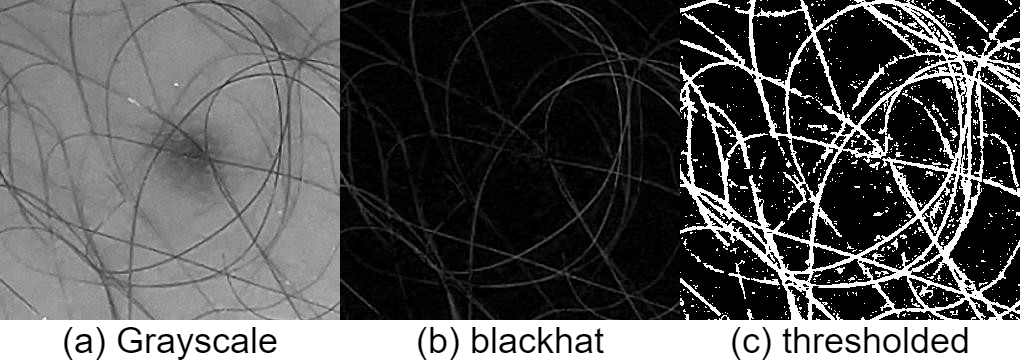
\includegraphics[scale=0.4]{figure/capitolo6/border1.png}
	\end{center}
	\caption{Preprocessing rimozione peli}	
\end{figure}
Il risultato finale è un immagine più fluida e pulita senza perdita di profondità.
\newline
\begin{figure}[h]
	\begin{center}
		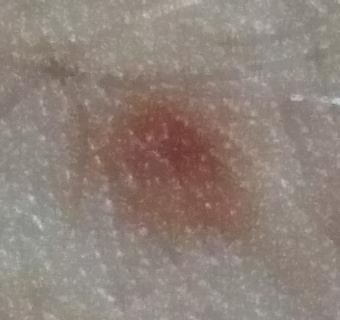
\includegraphics[scale=0.4]{figure/capitolo6/border2.jpg}
	\end{center}
	\caption{Immagine post preprocessing rimozione peli}	
\end{figure}
\newpage
\subsection{Image Segmentation}
L'obiettivo di questa elaborazione è separare il nevo dalla pelle.
\newline
La segmentazione delle immagini è una delle tecniche di base dell'image processing e della artificial vision. 
In generale, è possibile definire la segmentazione di una immagine come un processo di partizionamento del frame in gruppi omogenei, in modo tale che ciascuna regione sia omogenea ma l'unione di due regioni adiacenti non sia omogenea. \cite{haralick1985image}
\newline
Il fine ultimo della segmentazione è quello quindi di delineare i bordi del nevo, rendendo ben visibile la sua conformazione ai fini dell'analisi del dermatologo e come input per la valutazione del classificatore.  \cite{schaefer2011colour}
\newline
Nel nostro caso, la rilevazione del melanoma dipende dalle caratteristiche delle lesioni cutanee; qualsiasi errore nella segmentazione dell'immagine, per trovare il confine della lesione, può influire notevolmente sulle caratteristiche della lesione come dimensione, regolarità, rotondità e altre;.
\newline
È stato notato che nessuno degli algoritmi di segmentazione sviluppati è generalmente applicabile a tutte le immagini e diversi algoritmi non sono ugualmente adatti per particolari applicazioni.
\newline
Inoltre, la rappresentazione di un'immagine viene modificata in qualcosa che è più significativo e più facile da analizzare e facilita la selezione di una regione di interesse.
La segmentazione delle immagini è considerata il primo passo nelle applicazioni di analisi delle immagini mediche e anche uno dei compiti più critici, per questa ragione è fondamentale che le fasi precedenti abbiano processato l'immagine correttamente.
\newline
L'obiettivo della ricerca in questa fase è trovare e testare un metodo efficace e appropriato degli approcci esistenti di segmentazione delle immagini.
\newline
È stato notato che nessuno degli algoritmi di segmentazione sviluppati è generalmente applicabile a tutte le immagini e non sono ugualmente adatti per particolari applicazioni. 
\newline
Ci sono comunque molti algoritmi già sviluppati nel campo della segmentazione delle immagini, due tecniche all'avanguardia nella segmentazione delle lesioni cutanee sono state discusse in alcuni importanti lavori correlati:
\begin{itemize}
	\item Metodo di Otsu
	\item Metodo di segmentazione dello spostamento medio
\end{itemize}
\newpage
\subsubsection{Metodo della soglia di Otsu}
Se assumiamo che il confine della lesione in una certa misura sia chiaramente definito e distinto dallo sfondo, allora l'utilizzo di un semplice approccio di sogliatura come il metodo di Otsu è sufficiente per convertire l'immagine in un binario e separare la lesione dallo sfondo.
\newline
Il metodo di Otsu è un approccio non parametrico per la soglia dell'istogramma globale \cite{liu2009otsu}.
\newline
È stato sviluppato per calcolare la soglia ottimale dall'istogramma dell'immagine. Uno dei vantaggi di questo metodo è la focalizzazione su approcci non parametrici, che supportano il processo di automatizzazione del rilevamento della lesione cutanea con l'applicazione mobile senza selezione o regolazione del livello di soglia dell'utente, quindi \textbf{il metodo Otsu è uno dei migliori metodi di soglia automatica}, il principio di base nel metodo Otsu è dividere l'immagine in due classi: gli oggetti e lo sfondo.
La soglia automatica si ottiene trovando la massima
varianza tra le due classi.
L'algoritmo è il seguente:
\begin{itemize}
	\item Sia I = $[1, L]$ l'intervallo di livelli in scala di grigi dell'immagine $\phi$ (x,y) e $p_i$ la probabilità di ciascun livello
	\item Il numero di pixel con livello di grigio \textit{i} indicato con $\varphi_i$ da una probabilità di livello di grigio \textit{i} in un'immagine come $p_i=\frac{\varphi_i}{N}$
	\item La soglia automatica t che divide l'intervallo in due classi C0 = [1,..., t] e C1 = [t + 1,..., L], le distribuzioni di probabilità del livello di grigio per le due classi sono C1 e C2
	\item La media per le classi C1 e C2 sono $\mu_1$ e $\mu_2$
	\item Sia $\mu_r$ la media complessiva dell'intera immagine. Ovviamente, sommando le parti, è facile mostrare che $\mu_T$ = $\beta_1\mu_1$ + $\beta_2\mu_2$ dove $\beta_1$ = $\sum_{i=1}^{t}p_i$ e $\beta_2=$ = $\sum_{i=t+1}^{L}p_i p_i$
	\item  Dalle statistiche risulta chiaro che la somma totale delle probabilità è sempre uguale a uno $\beta_1 + \beta_2$ = 1
	\item Otsu ha definito la varianza tra classi di due classi C1 e C2 come
		\begin{equation}
		p^2=\beta_1(\mu_1 - \mu_t)^2+\beta_2(\mu_2-\mu_t)^2
		\end{equation}
	\item La soglia ottimale t è il valore che massimizza la varianza tra classi è $\sigma^2$
		\begin{equation}
		t=\max\{\sigma^2(t)\},1\leq t < L
		\end{equation}
\end{itemize}
\newpage
\subsubsection{Metodo di Segmentazione Mean Shift}
Nella sezione precedente, abbiamo ipotizzato che la lesione sia chiaramente definita e non è sempre così. Pertanto, viene proposto un algoritmo di segmentazione più accurato, chiamato \textit{clustering dei pixel}, che presenta i seguenti vantaggi:
\newline 
in primo luogo si basa sul colore dei pixel, sull'intensità e sulla posizione, o su una combinazione ponderata di questi fattori non solo sull'intensità del colore.
\newline
In secondo luogo, abbiamo più di due regioni considerate nel metodo; questo può aiutare nel caso di bordi sfocati o in presenza di rumore nella pelle.
\newline
Uno degli algoritmi di clustering più semplici è l'algoritmo K-means. 
\newline 
Il K-means è una tecnica iterativa utilizzata per partizionare un'immagine in K cluster e selezionare K cluster center, in modo casuale o in base a qualche euristica. 
\newline
L'algoritmo K-means non è appropriato per il caso studio, poiché l'obiettivo è utilizzare un algoritmo non parametrico automatizzato.
\newpage
\subsection{Estrazione del contorno}
Dopo aver segmentato l'immagine è possibile procedere ad una operazione di chiusura morfologica per rimuovere i piccoli spazi vuoti all'interno della lesione, quindi i contorni sono pronti per l'estrazione. 
\newline
"\textit{Un contorno è un elenco di punti che rappresentano, in un modo o nell'altro, una curva in un'immagine. Questa rappresentazione può essere diversa a seconda della circostanza in questione}" \cite{bradski2008learning}.
L'implementazione dell'estrazione del contorno utilizzata dalla libreria OpenCV utilizza un algoritmo che costruisce il bordo \cite{suzuki1985topological} grazie a sequenze di vertici (cioè Punti).
\newline
Il problema con questo metodo si ha quando l'immagine ha diverse sfumature di luce o ci sono più contorni selezionabili (in questo caso viene considerato il contorno più grande che non sempre contiene il nevo).
\newline
La soluzione proposta a questo problema è di filtrare le aree dei contorni, che sono più grandi di due terzi o più piccoli dei 10 pixel che quindi potrebbero essere un rumore e possono essere trascurate. 
\newline
Il seguente algoritmo viene utilizzato per selezionare il contorno della lesione dall'elenco dei contorni se il primo è maggiore di due terzi dell'intera immagine:
\begin{enumerate}
	\item Se ci sono più contorni nell'immagine, salvali in una lista
	\item Ordina i contorni nella lista e rimuovi i contorni più piccoli di 10 pixel e più larghi di 2/3 dell'immagine.
	\item Trova il massimo dei contorni
	\item Salva il contorno in una lista.
\end{enumerate}
Alla fine di questo processo è possibile disegnare il contorno sul nevo ed inoltre viene costruita un ellisse utilizzata come riferimento per le prossime analisi. Figura 5.5 (d)
	\begin{figure}[h]
	\begin{center}
		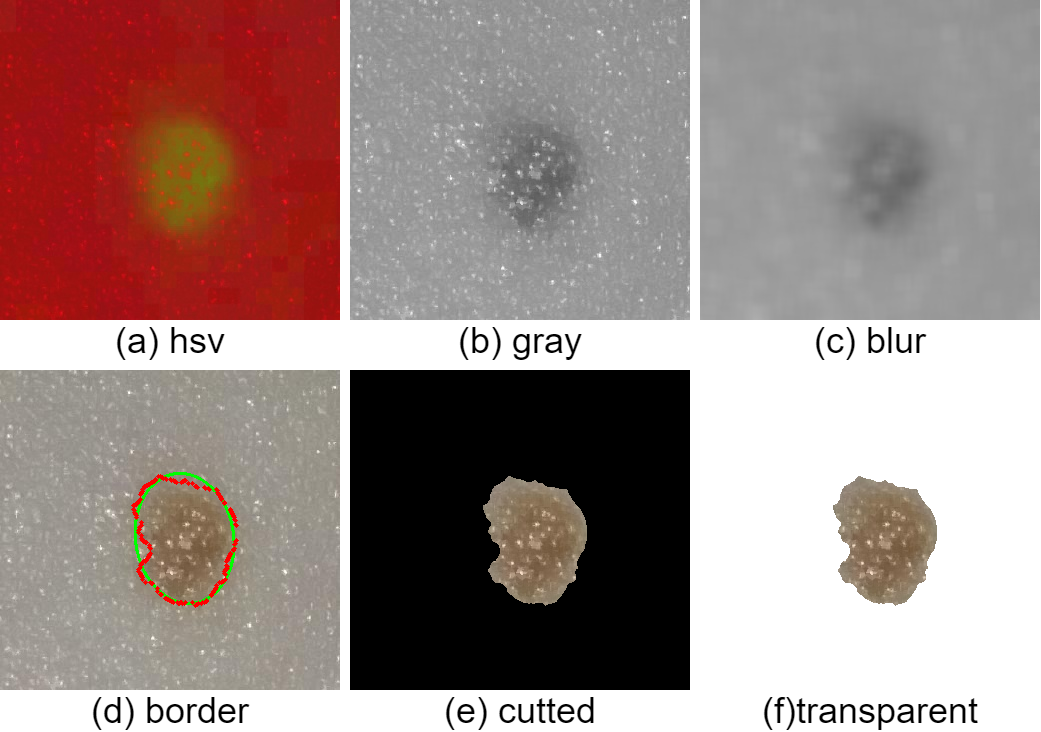
\includegraphics[scale=0.4]{figure/capitolo6/borderlist.png}
	\end{center}
	\caption{Fasi di preprocessing (Segmentazione, (a-c,e), Contorni (d))}	
\end{figure}
\subsection{Rimozione del nero}
L'ultima fase del preprocessing del nevo prima dell'estrazione delle feature e dell'analisi con il classificatore è la rimozione del nero (dato dalla segmentazione) dall'immagine.
L'algoritmo utilizzato per questa operazione è estremamente semplice:
\begin{itemize}
	\item Verifica i pixel che hanno colore nero [0, 0, 0]
	\item Converte i pixel neri in trasparenti [255, 255, 255, 0]
\end{itemize}
	\begin{figure}[h]
	\begin{center}
		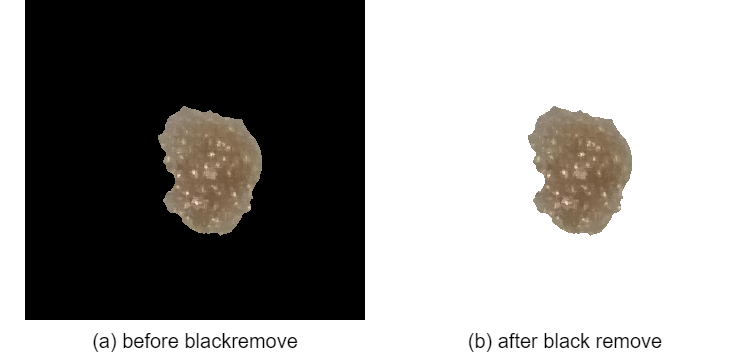
\includegraphics[scale=0.5]{figure/capitolo6/blackremove.png}
	\end{center}
	\caption{Prima e dopo l'esecuzione dell'algoritmo \textbf{black remove}}	
\end{figure}
\newpage

\section{Feature Extraction}
Dopo aver processato l'immagine correttamente è possibile procedere con l'estrazione delle caratteristiche del nevo utilizzando il metodo ABCD e aggiungendo anche altre informazioni inerenti la posizione del centroide, la visione 3D del nevo in 2D photometric stereo e la dimensione frattale. 
\subsection{Asimmetria/Simmetria}
Un nevo benigno è generalmente circolare o comunque rotondo, il melanoma è irregolare e di dimensioni maggiori; per questo motivo l'asimmetria di una lesione è di fondamentale importanza nella diagnosi. 
\newline
La lesione è generalmente contenuta in una macchia più grande. I dermatologi valutano l'asimmetria confrontando le due metà della lesione sfruttando l'asse principale come riferimento.
\newline
Per la rilevazione computazionale dell'asimmetria, esistono diversi algoritmi in letteratura.
\newline
Un possibile algoritmo per il calcolo dell'asimmetria \cite{stoecker2005detection} prevede il calcolo A=$\frac{Dist}{\sqrt{Area}}$ dove Dist è la distanza Euclidea tra il centroide e il punto più lontano, e trai il centroide della lesione fratto l'area della lesione.
\newline
In questa tesi è stato utilizzato un algoritmo che prende in input l'immagine segmentata e costruisce i contorni del nevo 4 punti di riferimento opposti tra loro, più un punto centrale (il centroide del nevo) e ne calcola il livello di asimmetria o simmetria.

\subsection{Bordo}
Per il calcolo del bordo esistono in letteratura diversi metodi.
\newline
Un riferimento principale per la valutazione del bordo è la sua circolarità.\cite{montero2009state}.
In questa attività di tesi è stato scelto di non calcolare l'irregolarità del bordo ma di lasciare al dermatologo la possibilità di visionare il contorno del nevo evidenziato di colore rosso, in modo da riuscire a vedere qualsiasi tipo di irregolarità.
\newline
Ad ogni modo analizziamo le possibile tecniche di calcolo dell'indice di irregolarità del bordo.
Uno studio di Maglogiannis et al. \cite{maglogiannis2005integrated} ha evidenziato la possibilità di calcolare l'\textbf{irregolarità del bordo} utilizzando la seguente formula:
		\begin{equation}
			Irregularity= \frac{P}{A}
		\end{equation}
Il rapporto dipende dalle dimensioni del melanoma, per questa ragione il calcolo può essere migliorato attraverso la seguente formula:
		\begin{equation}
			Irregularity= \frac{P}{Diametro Maggiore}
		\end{equation}
Un altro metodo per il calcolo dei bordi è Hull/Contour Ratio (HCR) \cite{ramlakhan2011mobile} basato sul rapporto tra il contorno dell'ellisse costruita sul melanoma ed il suo perimetro.
}
\newpage
\subsection{Colore}
Una delle prime caratteristiche di un melanoma è il colore e la varianza di colore, le lesioni da melanoma hanno infatti elementi marroni o neri in base alla produzione di melanina e al tipo di pelle.
\newline
Per questa motivazione è stato implementato un algoritmo per l'estrazione di cluster di colori \cite{faziloglu2003colour}, in questo modo il dermatologo ha la possibilità di vedere quali sono i colori che hanno una maggior presenza nel melanoma.
\newline
L'algoritmo esegue i seguenti passi:
\begin{enumerate}
	\item Prende in input un numero n (5 nel nostro caso di studio) di cluster nel quale inserire i colori.
	\item Analizza i singoli pixel del nevo ed inserisce nel cluster i pixel che hanno lo stesso colore o colore simile.
	\item Per ogni cluster costruisce un rettangolo con il colore e stampa la percentuale per ogni colore.
\end{enumerate}
Il risultato di questo algoritmo è una barra di n colori (in base al numero di cluster che si danno in input) in RGB. 
	\begin{figure}[h]
	\begin{center}
		
\includegraphics[scale=0.5]{figure/capitolo6/color.png}
	\end{center}
	\caption{Scala di colori prodotta dall'applicazione \textbf{color}}	
	\end{figure}
\newpage
\subsection{Dimensione Frattale}
Il reticolo pigmentario è un parametro di analisi molto importante, le linee della rete corrispondono alle creste epidermiche allungate e gli spazi della rete alle papille dermiche; nelle lesioni benigne, il reticolo pigmentario appare regolare e sfumato alla periferia, mentre nelle lesioni sospette appare irregolare a maglie grossolane, con pigmentazione di varia intensità, non ombreggiato alla periferia e asimmetrico.
Lo pseudoreticolo pigmentario è un'interruzione della pigmentazione da macchie ipopigmentate determinate dai follicoli piliferi e sbocchi ghiandolari. Una lesione maligna per via degli atipici melanociti aumentati di numero, appare irregolare e grossolana [4].
\newline
La dimensione frattale permette di calcolare la ripetizione di ogni sotto-struttura, questa funzione può essere fatto facilmente grazie all'analisi basata su colore analizzata in precedenza, dove ogni sotto-struttura viene inserita in un cluster.
\newpage
\subsection{Diametro}
Il melanoma tende a crescere di più dei nevi comuni, specialmente quelli con un diametro di 6 mm.
In genere, una lesione sospetta ha un diametro > 6 mm \cite{rigel2010evolution}, ma studi recenti hanno dimostrato che, con l'aumento del diametro del melanoma, aumenta anche la profondità di Breslow e che circa il 30\% delle lesioni inferiori a 6 mm sono comunque invasive.
A causa delle forme irregolari della lesione, per riuscire a calcolare il diametro viene costruito un rettangolo sull'ellisse del nevo e vengono tracciati, come riferimenti sui lati del rettangolo, il punto centrale della base e il punto centrale dell'altezza, a questo punto congiungendo i punti dei cateti paralleli si hanno diametro minimo e massimo del nevo.
\newline
Attraverso i due diametri è possibile calcolare il diametro del nevo con i seguente rapporto:
\begin{equation}
	Diametro Assoluto=\frac{dA+dB}{2}
\end{equation}
dove dA è il diametro maggiore e dB il diametro minore.
\newline
Il valore prodotto da questa funzione non è sufficiente a dare informazioni relative al nevo ma solo assolute e che dipendono fortemente dal frame dato in input; per cui, per dare una semantica alle informazioni, è necessario conoscere a che distanza si trova la camera.
\newline
Nei nuovi dispositivi dotati di sensori ad infrarossi per il calcolo della profondità il problema è di semplice risoluzione, ma con uno smartphone comune il problema è di notevole entità.
\newline
Una possibile soluzione è la divisione dei diametro dA e dB per il valore di zoom inserito per effettuare la foto, e il valore di una costante pari a 100 (Non ci sono riferimenti scientifici a sostegno di questa affermazione, ma diverse prove effettuate su nevi hanno dato risultati soddisfacenti)
\begin{equation}
	Diametro=(Diametro Assoluto/zoom)/const
\end{equation}
I passi visibili per il calcolo del diametro assoluti sono in Figura 5.8
	\begin{figure}[h]
	\begin{center}
		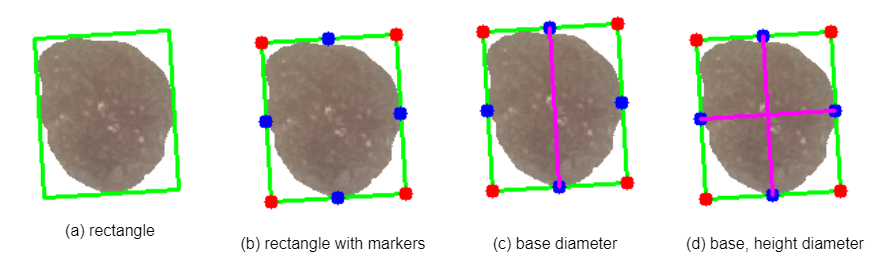
\includegraphics[scale=0.47]{figure/capitolo6/diameter.png}
	\end{center}
	\caption{Passi per il calcolo del \textbf{diametro}}	
\end{figure}
Un'altro indice utilizzabile per migliorare la precisione nel calcolo del diametro è la caratteristica focale dell'immagine, ovvero il calcolo del blur della frame, potrebbe offrire un ulteriore riferimento nel calcolo del diametro; purtroppo in letteratura non ci sono riferimenti in tal senso.
\newpage
\subsection{2D Photometric Stereo}
Un'ultima caratteristica visiva peculiare del melanoma è l'elevazione palpabile della lesione. 
\newline
Questa caratteristica viene valutata dal medico con il tatto, ma non è ancora considerata negli strumenti software, né simulata- 
\newline
La comparsa di una papula o di un nodulo nel contesto di una lesione pigmentata può spesso denotare la presenza di una lesione maligna, che è rilevabile solo palpando il melanoma.
\newline
Per questo motivo è stato adottato un algoritmo 2D photometric stereo per misurare il grado di elevazione della lesione, in maniera visiva, dando la sensazione al dermatologo di vedere in 3D il melanoma.
\newline
Il photometric stereo (utilizzato in molte applicazioni di ricostruzione 3D) è un metodo per stimare la profondità e l'orientamento della superficie di immagini, della stessa vista prese da direzioni diverse \cite{xie2016deep3d} e si basa su costruzioni normali basate sulla direzione della luce.

\textbf{Il photometric stereo} è una tecnica che stima la profondità e l'orientamento della superficie da immagini della stessa vista prese da direzioni diverse e quindi con diverse angolazioni di luce.
\newline
Teoricamente, solo tre direzioni sono sufficienti per ottenere le normali, ma per ridurre al minimo i rumori insiti nel processo, spesso è richiesto un numero superiore al minimo per immagini realistiche. \cite{verma1999photometric}
\newline
Questo metodo, tuttavia, presenta alcune limitazioni:
\begin{enumerate}
	\item La sorgente luminosa deve essere lontana dagli oggetti
	\item Macchie speculari o scure nelle regioni non danno risultati soddisfacenti
	\item le ombre devono essere mascherate per garantire una valida ricostruzione della superficie 3D.
\end{enumerate}
Il primo passo nei calcoli della normal map è calibrare la sorgente di luce, cioè stimare la direzione della luce.
\newline
Un modo per farlo è utilizzare la sfera cromata su cui viene utilizzato il punto più luminoso per identificare la direzione della luce.
\begin{figure}[h]
	\begin{center}
		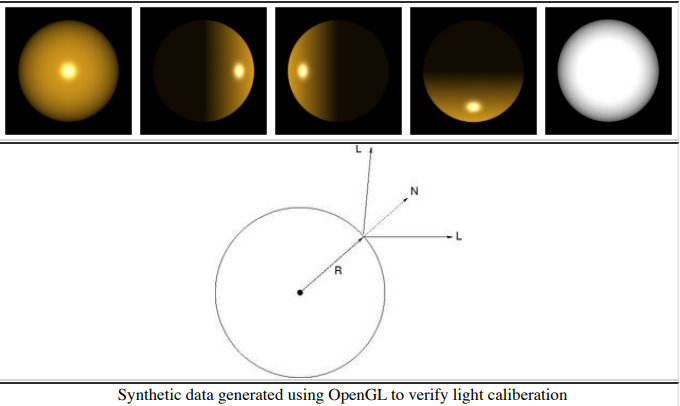
\includegraphics[scale=0.5]{figure/capitolo4/sphere.png}
	\end{center}
	\caption{Direzione della luce sulla sfera }	
\end{figure}
		\begin{equation}
		L=2(N.R)N-R
		\end{equation}
Dove R è la direzione di riflessione presa come [0,0,1]. [Px, Py] è la posizione del punto più luminoso sull'immagine e [Cx, Cy] è il centro del cromo nello spazio dell'immagine che può essere stimato dalla maskimage/.
\newline
Per le superfici Lambertain, l'intensità in qualsiasi punto della superficie può essere rilevata dall'equazione
\begin{equation}
		I=k_dN.L
\end{equation}
Dove N è la normale alla superficie ed L è la direzione della luce riflessa.
\newline
Per determinare N, abbiamo bisogno di almeno tre sorgenti luminose che non si trovano sullo stesso piano.
\newline
Pertanto, possiamo recuperare sia la mappa normale che quella dell'albedo per pixel, se il pixel riceve luce da almeno una sorgente.
\newline
Alla fine ci sono molti pixel nella regione in cui l'intensità della luce proveniente dalle sorgenti è molto bassa, quindi dobbiamo saltare quei pixel per i calcoli.
A questo punto possiamo calcolare l'immagine 3D nel nevo in 2D photometric stereo come visibile nella Figura 5.10
\newpage
\begin{figure}[h]
	\begin{center}
		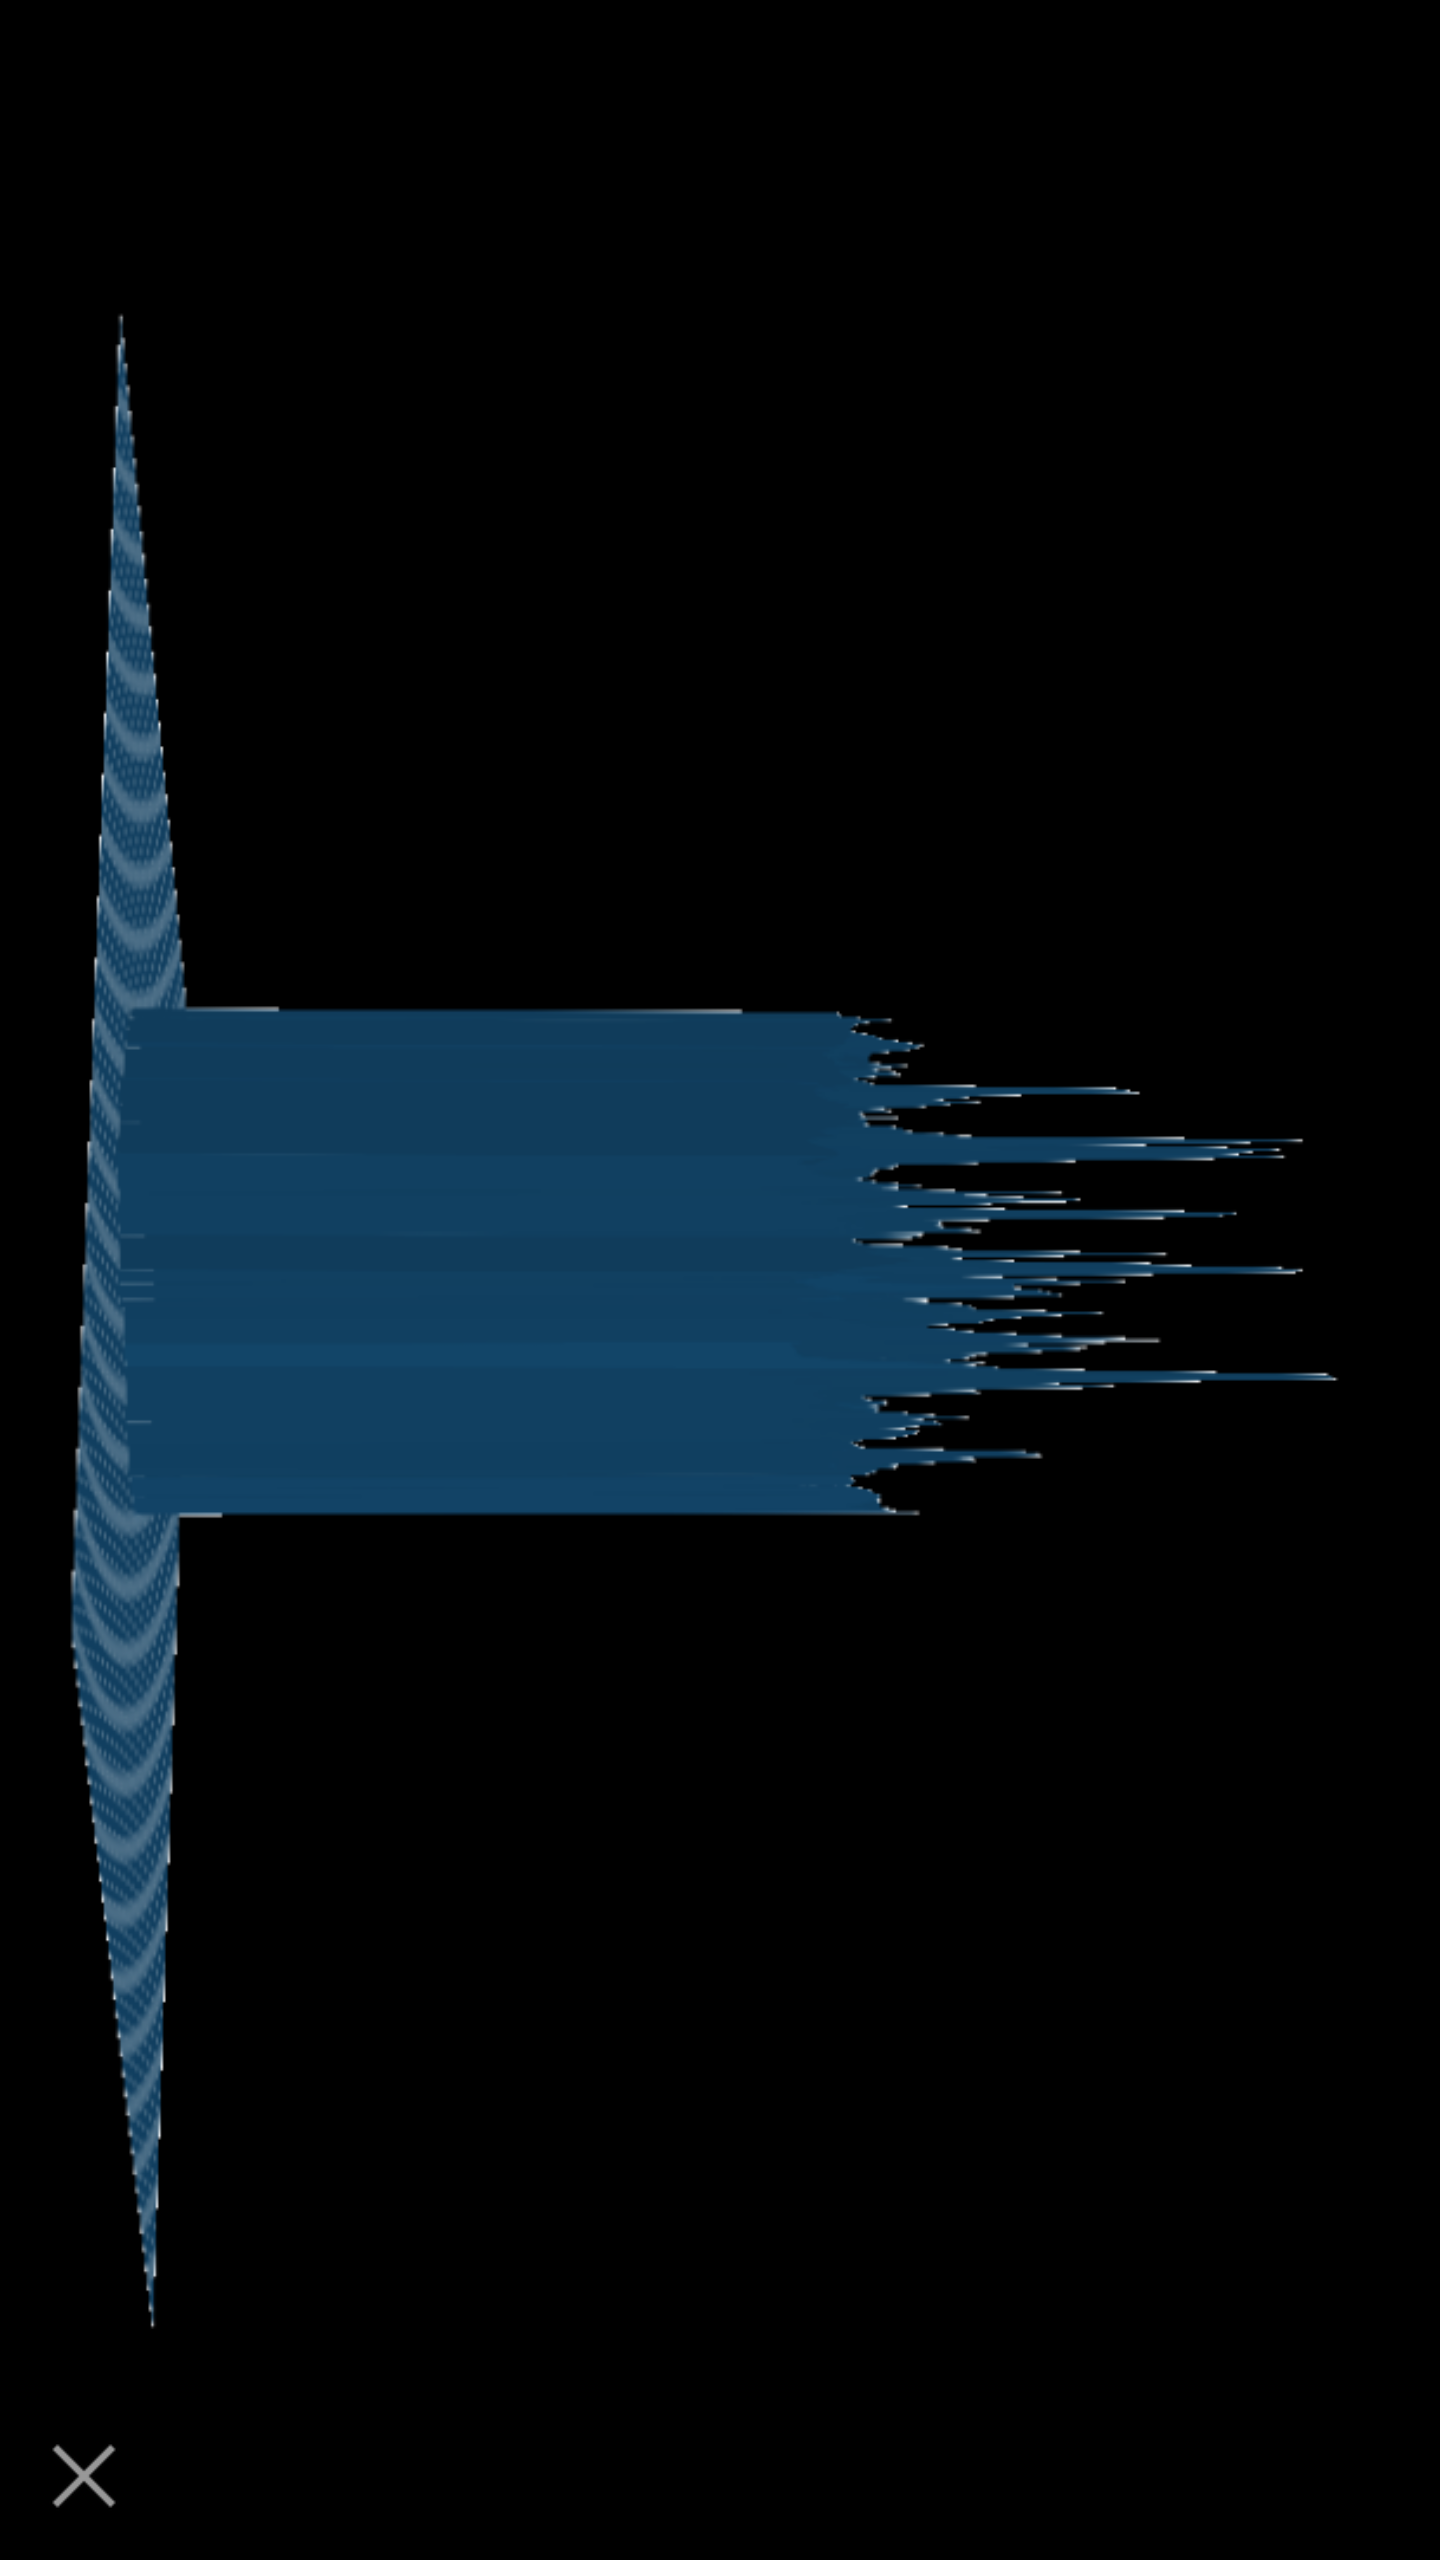
\includegraphics[scale=0.1]{figure/capitolo6/3d.png}
	\end{center}
	\caption{Immagine del nevo in \textbf{2D photometric stereo}}	
\end{figure}
\newpage
\section{Classificazione del Melanoma}
Per la classificazione e valutazione del melanoma è stato utilizzato il classificatore h5 descritto nel capitolo precedente.
L'obiettivo di questa fase è fornire al dermatologo una valutazione aggiuntiva per l'analisi del melanoma. Il classificatore è stato progettato per fornire un valore binario di valutazione con un valore di accuratezza da 0 a 1 per una migliore comprensione da parte del medico.
È stato scelto di far mostrare nell'applicazione solo il valore di accuratezza dell'analisi, poiché un valore binario avrebbe fornito una valutazione troppo approssimata dell'analisi. In questo modo, in base al grado di fiducia fornito, il dermatologo può fornire una valutazione positiva o negativa sul nevo analizzato.
\newpage
\section{Visualizzazione in Realtà Aumentata}
L'applicazione ha lo scopo di supportare il dermatologo nell'analisi dei melanomi visualizzando in realtà aumentata le informazioni fornite dalla fase di estrazione delle caratteristiche descritta nella sezione precedente.\cite{francese2020}
Alcune delle caratteristiche che l'applicazione ha sono:
\begin{itemize}
	\item Centratura e selezione delle lesioni cutanee
	\item Visione del Classificatore CNN
	\item Aggiornamento in tempo reale delle informazioni in realtà aumentata.
\end{itemize}
Un'applicazione demo che implementa tali caratteristiche è stata creata per questo progetto di tesi, e descritta nei capitoli successivi.
